% Options for packages loaded elsewhere
\PassOptionsToPackage{unicode}{hyperref}
\PassOptionsToPackage{hyphens}{url}
%
\documentclass[
]{book}
\usepackage{amsmath,amssymb}
\usepackage{lmodern}
\usepackage{iftex}
\ifPDFTeX
  \usepackage[T1]{fontenc}
  \usepackage[utf8]{inputenc}
  \usepackage{textcomp} % provide euro and other symbols
\else % if luatex or xetex
  \usepackage{unicode-math}
  \defaultfontfeatures{Scale=MatchLowercase}
  \defaultfontfeatures[\rmfamily]{Ligatures=TeX,Scale=1}
\fi
% Use upquote if available, for straight quotes in verbatim environments
\IfFileExists{upquote.sty}{\usepackage{upquote}}{}
\IfFileExists{microtype.sty}{% use microtype if available
  \usepackage[]{microtype}
  \UseMicrotypeSet[protrusion]{basicmath} % disable protrusion for tt fonts
}{}
\makeatletter
\@ifundefined{KOMAClassName}{% if non-KOMA class
  \IfFileExists{parskip.sty}{%
    \usepackage{parskip}
  }{% else
    \setlength{\parindent}{0pt}
    \setlength{\parskip}{6pt plus 2pt minus 1pt}}
}{% if KOMA class
  \KOMAoptions{parskip=half}}
\makeatother
\usepackage{xcolor}
\IfFileExists{xurl.sty}{\usepackage{xurl}}{} % add URL line breaks if available
\IfFileExists{bookmark.sty}{\usepackage{bookmark}}{\usepackage{hyperref}}
\hypersetup{
  pdftitle={A Minimal Book Example},
  pdfauthor={John Doe},
  hidelinks,
  pdfcreator={LaTeX via pandoc}}
\urlstyle{same} % disable monospaced font for URLs
\usepackage{longtable,booktabs,array}
\usepackage{calc} % for calculating minipage widths
% Correct order of tables after \paragraph or \subparagraph
\usepackage{etoolbox}
\makeatletter
\patchcmd\longtable{\par}{\if@noskipsec\mbox{}\fi\par}{}{}
\makeatother
% Allow footnotes in longtable head/foot
\IfFileExists{footnotehyper.sty}{\usepackage{footnotehyper}}{\usepackage{footnote}}
\makesavenoteenv{longtable}
\usepackage{graphicx}
\makeatletter
\def\maxwidth{\ifdim\Gin@nat@width>\linewidth\linewidth\else\Gin@nat@width\fi}
\def\maxheight{\ifdim\Gin@nat@height>\textheight\textheight\else\Gin@nat@height\fi}
\makeatother
% Scale images if necessary, so that they will not overflow the page
% margins by default, and it is still possible to overwrite the defaults
% using explicit options in \includegraphics[width, height, ...]{}
\setkeys{Gin}{width=\maxwidth,height=\maxheight,keepaspectratio}
% Set default figure placement to htbp
\makeatletter
\def\fps@figure{htbp}
\makeatother
\setlength{\emergencystretch}{3em} % prevent overfull lines
\providecommand{\tightlist}{%
  \setlength{\itemsep}{0pt}\setlength{\parskip}{0pt}}
\setcounter{secnumdepth}{5}
\usepackage{booktabs}
\ifLuaTeX
  \usepackage{selnolig}  % disable illegal ligatures
\fi
\usepackage[]{natbib}
\bibliographystyle{plainnat}

\title{A Minimal Book Example}
\author{John Doe}
\date{}

\begin{document}
\maketitle

{
\setcounter{tocdepth}{1}
\tableofcontents
}
\hypertarget{section}{%
\chapter{}\label{section}}

Modern challenges of reproducibility in research, particularly computational reproducibility {[}cite{]}, have produced a lot of discussion in papers, blogs and videos, some of which are listed \href{https://github.com/davan690/reproducible-guidebook/blob/main/sections/references/index.md}{here}.

In this short introduction, we briefly summarise some of the principles, definitions and questions relevant to reproducible research that have emerged in the literature. We outline basic and widely applicable steps for promoting reproducibility. While our suggestions for tools and workflow are aimed primarily at the computational environment of the R programming language, the principles and definitions sketched out here are applicable to researchers working in any environment.

You are welcome to contribute to the original guide (fix typos, add to the \href{https://github.com/ropensci/reproducibility-guide/blob/gh-pages/sections/references/index.md}{reference list}, etc.) by submitting a pull request to its \href{https://github.com/ropensci/reproducibility-guide}{github repository}. Or contact me with regard to this extended guide here \url{https://github.com/davan690/reproducible-guidebook}.

If you're not familiar with R, have a look at \href{http://rforcats.net/}{rforcats.net} for a gentle introduction, and if you're already working with R then have a look at Hadley's \href{http://adv-r.had.co.nz/}{Advanced R programming book} for a guide to best practices.

\hypertarget{why-do-reproducible-research}{%
\section{Why do reproducible research?}\label{why-do-reproducible-research}}

There are two basic reasons to be concerned about making your research reproducible. The first is \textbf{to show evidence of the correctness of your results}. Descriptions contained in scholarly publications are rarely sufficient to convince sceptical readers of the reliability of our work. In simpler times, scholarly publications showed the reader most of the work involved in getting the result. The reader could make an informed choice about the credibility of the science. Now, the reader may feel they are being asked to blindly trust in all the details that were not described in the original journal article.

Adopting a reproducible workflow means providing our audience with the code and data that demonstrates the decisions we made as we generated our results. This makes it easier for others to satisfy themselves that our results are reliable (or not, since reproducibility is no guarantee of correctness).

The second reason to aspire to reproducibility is \textbf{to enable others to make use of our methods and results}. Equipped with only our published article, our colleagues might struggle to reconstruct our method in enough detail to apply it to their own data. Adopting a reproducible workflow means publishing our code and data in order to allow our colleagues to extend our approach to new applications with a minimum of effort. This has the potential to save a great deal of time in transmitting knowledge to future researchers.

\hypertarget{what-are-the-principles-of-reproducible-research}{%
\section{What are the principles of reproducible research?}\label{what-are-the-principles-of-reproducible-research}}

The motivating principle for reproducible research is that the traditional unit of scholarly communication - a published article - is only the tip of the iceberg of the research process. Jon Claerbout described the article as merely an advertisement for research \href{http://sepwww.stanford.edu/doku.php?id=sep:research:reproducible:seg92}{(Claerbout and Karrenbach 1992)}:

\begin{quote}
An article about computational results is advertising, not scholarship. The actual scholarship is the full software environment, code and data, that produced the result.
\end{quote}

In most cases, when we have only an article, we are unable to engage with the bulk of the details and decisions that lead to the figures, tables and narrative presented in the article.

The aim of practising reproducible computational research is to expose more of the research workflow to our audience. This makes it easier for them to make a more informed assessment of our methods and results, and makes it easier for them to adapt our methods to their own research.

\hypertarget{what-are-the-different-kinds-of-reproducible-research}{%
\section{What are the different kinds of reproducible research?}\label{what-are-the-different-kinds-of-reproducible-research}}

Enabling reproducibility can be complicated, but by separating out some of the levels and degrees of reproducibility the problem can become more manageable because we can focus our efforts on what best suits our specific scientific domain. Victoria Stodden \href{http://edge.org/response-detail/25340}{(2014)}, a prominent scholar on this topic, has identified some useful distinctions in reproducible research:

\begin{itemize}
\item
  \emph{Computational reproducibility}: when detailed information is provided about code, software, hardware and implementation details.
\item
  \emph{Empirical reproducibility}: when detailed information is provided about non-computational empirical scientific experiments and observations. In practise this is enabled by making data freely available, as well as details of how the data was collected.
\item
  \emph{Statistical reproducibility}: when detailed information is provided about the choice of statistical tests, model parameters, threshold values, etc. This mostly relates to pre-registration of study design to prevent p-value hacking and other manipulations.
\end{itemize}

\href{http://stodden.net/icerm_report.pdf}{Stodden et al.~(2013)} place \textbf{computational reproducibility} on a spectrum with five categories that account for many typical research contexts:

\begin{quote}
\begin{itemize}
\tightlist
\item
  \emph{Reviewable Research}. The descriptions of the research methods can be independently assessed and the results judged credible. (This includes both traditional peer review and community review, and does not necessarily imply reproducibility.)
\item
  \emph{Replicable Research}. Tools are made available that would allow one to duplicate the results of the research, for example by running the authors' code to produce the plots shown in the publication. (Here tools might be limited in scope, e.g., only essential data or executables, and might only be made available to referees or only upon request.)
\item
  \emph{Confirmable Research}. The main conclusions of the research can be attained independently without the use of software provided by the author. (But using the complete description of algorithms and methodology provided in the publication and any supplementary materials.)
\item
  \emph{Auditable Research}. Sufficient records (including data and software) have been archived so that the research can be defended later if necessary or differences between independent confirmations resolved. The archive might be private, as with traditional laboratory notebooks.
\item
  \emph{Open or Reproducible Research}. Auditable research made openly available. This comprised well-documented and fully open code and data that are publicly available that would allow one to (a) fully audit the computational procedure, (b) replicate and also independently reproduce the results of the research, and (c) extend the results or apply the method to new problems.
\end{itemize}
\end{quote}

This kind of spectrum is valuable because it easy for us to understand how our current practices can be defined. It helps to pinpoint limitations that we face (for example many researchers are unable to publicly release sensitive data) and identify basic changes we can make to improve reproducibility.

\hypertarget{how-can-software-tools-can-make-our-research-more-reproducible}{%
\subsubsection{How can software tools can make our research more reproducible?}\label{how-can-software-tools-can-make-our-research-more-reproducible}}

For many domains of science there are already several options for software tools to help overcome the technical challenges of doing reproducible research. These tools enable researchers to capture and communicate the details of their workflow with much greater efficiency that simply writing a lengthy prose narrative. There are three general types of software tools (cf.~\href{http://stodden.net/icerm_report.pdf}{Stodden et al 2013}). For more specific details on the tools named here, see our \href{http://ropensci.github.io/reproducibility-guide/sections/tools/}{tools page}:

\begin{itemize}
\item
  \textbf{Literate computing, authoring, and publishing}. These tools enable writing and publishing self-contained documents that include narrative and code used to generate both text and graphical results. In the R ecosystem, \href{http://yihui.name/knitr/}{knitr} and its ancestor \href{http://www.stat.uni-muenchen.de/~leisch/Sweave/}{Sweave} used with \href{https://www.rstudio.com/}{RStudio} are the main tools for literate computing. \href{http://daringfireball.net/projects/markdown/}{Markdown} or \href{http://www.latex-project.org/}{LaTeX} are used for writing the narrative, with chunks of R code sprinkled throughout the narrative. \href{http://ipython.org/}{IPython} is a popular related system for the Python language, providing an interactive notebook for browser-based literate computing.
\item
  \textbf{Version control}. These tools enable you to keep a record of file changes over time, so specific versions can be recalled later. During exploratory data analysis you might pursue several paths that lead nowhere, with version control you can efficiently revert to an earlier point in the analysis without starting from scratch. There are several systems that are widely used, and amongst R users the \href{http://git-scm.com/}{git} version control system is especially popular. Version control tools combined with web services such as \href{https://github.com/}{Github} and \href{https://bitbucket.org/}{BitBucket} also enable you to work with collaborators with a minimum of confusion and friction.
\item
  \textbf{Tracking provenance}. Provenance refers to the tracking of chronology and origin of research objects, such as data, source code, figures, and results. Programs that track provenance enable you to capture a complex workflow that relies on many different tools. Tools that record provenance of computations include \href{http://www.vistrails.org/}{VisTrails}, \href{https://kepler-project.org/}{Kepler}, \href{http://www.taverna.org.uk/}{Taverna}, and several others. Many of these can include R as part of a sequence of tools. If your workflow uses many different programs, these provenance trackers will be useful for efficiently documenting the order of processes and parameters to show others your analytical process.
\item
  \textbf{Automation} Several Unix tools are useful for streamlined automation and documentation of the research process, e.g.~editing files, moving input and output between different parts of your workflow, and compiling documents for publication. Scripts for \href{http://www.gnu.org/software/bash/}{shell programs} and \href{http://www.gnu.org/software/make/}{make} files enable highly efficient and easily repeatable control of your computer. These scripts can also be used to keep a record of every kind of action on your computer. There are lots of options for learning and using Unix tools, for more details check out Karl Broman's \href{http://kbroman.github.io/Tools4RR/assets/lectures/02_unix_withnotes.pdf}{list of tools and editors} for different platforms.
\item
  \textbf{Capturing the computational environment} A substantial challenge in reproducing analyses is installing and configuring the web of dependencies of specific versions of various analytical tools. Virtual machines (a computer inside a computer) enable you to efficiently share your entire computational environment with all the dependencies intact. Popular VM applications include \href{https://www.virtualbox.org/}{VirtualBox} and \href{http://www.vmware.com/}{VMWare}. One challenge of working with VMs is that the files that contain the environment are not small, typically one gigbyte or more, which can be awkward to share. On the other hand, they are convenient for use with cloud-based services such as Amazon EC2.
\end{itemize}

\hypertarget{how-to-give-and-receive-credit-for-reproducible-research}{%
\subsubsection{How to give and receive credit for reproducible research?}\label{how-to-give-and-receive-credit-for-reproducible-research}}

One of the challenges going forward is how to share code and data. In many disciplines, researchers have concerns about copyright, being scooped, and getting recognition for the effort invested in writing code and collecting data. These concerns hinder people from sharing details of their research and impede reproducibility. In response to these concerns, \href{http://papers.ssrn.com/sol3/papers.cfm?abstract_id=1362040}{Stodden (2009)} has proposed the \textbf{Reproducible Research Standard} to encourage researchers to release their products with standardised instructions for reuse and attribution. In brief, this standard recommends that researchers:

\begin{enumerate}
\def\labelenumi{\arabic{enumi}.}
\tightlist
\item
  Release media components (text and figures, such as markdown, LaTeX, PDF and other documents) under a \href{http://creativecommons.org/licenses/by/4.0/}{Creative Commons Attribution (CC-BY) licence}.
\item
  Release code components under the \href{http://opensource.org/licenses/MIT}{MIT license} or similar.
\item
  Release data under the \href{https://creativecommons.org/publicdomain/zero/1.0/}{CC0 licence}, that is, place data in the public domain.
\end{enumerate}

There are several options for depositing these components of the research compendia online that give \href{https://en.wikipedia.org/wiki/Digital_object_identifier}{DOI}s for convenient citing and discovery (eg. \href{http://figshare.com/}{figshare} with github integration, \href{https://zenodo.org/}{zenodo} also with github integration, and \href{http://researchcompendia.org/}{researchcompendia.org}).

These recommendations will not be suitable for every occasion. For example, research that uses human subjects data obviously cannot make that data publicly available without substantial changes to protect identities. In these situations, some modifications will be required to maximize reproducibility while honoring obligations to stakeholders. In some cases, a solution might be releasing a sample of ``dummy'' data that contains similar qualities to the real data set. While this would not be fully `reproducible research' as defined above, it would still be very useful to other researchers who could use a validated sample to inspect, evaluate and extend the research.

\hypertarget{how-can-we-make-reproducible-research-the-norm}{%
\subsubsection{How can we make reproducible research the norm?}\label{how-can-we-make-reproducible-research-the-norm}}

There are substantial costs of time and effort involved in become familiar with ways of making your research more reproducible. Until code and data sharing becomes common practice, it can be difficult for many researchers to see the point of adopting these procedures. There are many small informal things we can do to promote reproducibility and increase recognition of these efforts. Along these lines, \href{http://www.stanford.edu/~vcs/papers/CiSE2012-LMS.pdf}{Leveque et al.~(2012)} recommend we:

\begin{quote}
\begin{itemize}
\tightlist
\item
  \textbf{Train students} by putting homework, assignments \& dissertations on the reproducible research spectrum
\item
  \textbf{Publish examples} of reproducible research in our field
\item
  \textbf{Request code \& data} when reviewing
\item
  \textbf{Submit to \& review for journals} that support reproducible research
\item
  \textbf{Critically review \& audit} data management plans in grant proposals
\item
  Consider reproducibility wherever possible in \textbf{hiring, promotion \& reference letters}.
\end{itemize}
\end{quote}

Similarly, \href{http://reproducibility.cs.arizona.edu/tr.pdf}{Collberg et al.~(2014)} summarise the lessons they learned in attempting to reproduce 600 computer science projects:

\begin{quote}
\begin{itemize}
\tightlist
\item
  Unless you have compelling reasons not to, plan to release the code. It is the right thing to do, and if you start with this mind-set from the beginning of the project, the amount of extra work will likely be negligible.
\item
  Students will leave, plan for it. When building the system keep in mind that the code should outlive both you and the student.
\item
  Create permanent email addresses. You and your students will most likely be changing jobs a few times during your career. While some schools will keep old email addresses around, or forward email, you cannot count on it. Create email addresses that you know will be permanent throughout your working life and use them in all professional correspondence.
\item
  Create project websites. These are more likely to remain functional over time than email addresses. Put the URL in the paper. Be prepared to upload code and test data to your web sites at the same time as you upload the paper describing your system to a conference site for review.
\item
  Use a source code control system. Whenever you submit or publish a paper, set a label on the corresponding code version so that you can easily recreate it.
\item
  Backup your code.
\item
  Resolve licensing issues. If you anticipate problems start the licensing process early, so that you are able to release the code at the same time as the paper is submitted for publication.
\item
  Keep your promises. If your grant application states that you will be sharing code with the community, plan for keeping that promise.
\item
  Plan for longevity. Projects may live on for a long time, with many students building on the code. Plan for this at the onset of the project, by setting up the appropriate directory structures, plug-in architectures, etc., which will allow the project to grow.
\item
  Avoid cool but unusual designs. Unless you have a compelling reason to do otherwise, stay with standard operating systems, programming languages, and tool chains.
\end{itemize}
\end{quote}

\hypertarget{whats-next}{%
\subsubsection{What's next?}\label{whats-next}}

If this is all news to you, the next steps are to simply dive in and find the tools and workflow that best suit your research domain. Incrementally adding reproducibility to current projects is an excellent way to learn more, and then future projects can be planned for built-in reproducibility from the start. Becoming involved in the community of researchers in your domain who are using tools for reproducibility can also ease the transition to new tools and workflows.

Read through the other \href{http://ropensci.github.io/reproducibility-guide/}{sections of this site} for more specific instructions, details and ideas on reproducible research using R. Also check out our curated list of \href{http://ropensci.github.io/reproducibility-guide/sections/references/}{further readings} which includes links to numerous excellent guides on the practical details of improving reproducibility with R.

\hypertarget{resources}{%
\chapter{Resources}\label{resources}}

Over the past few years there has been a hige development of reproducible research tools using R.

\hypertarget{rstudio-tools-and-packages}{%
\section{RStudio tools and packages}\label{rstudio-tools-and-packages}}

Since the development of R and RStudio (and a magnitude of other IT changes happening at the same time) there are now tools for working with issues to do with \href{https://www.nature.com/news/1-500-scientists-lift-the-lid-on-reproducibility-1.19970}{reproducibility}. There are many blogs from a simple web search.

Here is a collection of the posts I have drawn inspiration from:

\begin{itemize}
\tightlist
\item
  \href{https://www.r-bloggers.com/reproducible-research-and-r-workflow/}{R bloggers post}: Jeromy Anglim
\item
  \href{https://cyberhelp.sesync.org/basic-git-lesson/2016/08/25/}{Reproducible workflows in RStudio}
\item
  \href{https://maraaverick.rbind.io/2017/09/r-workflow-fun/}{R workflow}: Mara Averick
\item
  \href{https://methodsblog.com/2016/10/05/reproducibility-with-r/}{Methods in Ecology}
\item
  \href{https://csgillespie.github.io/efficientR/workflow.html}{workflow general tips}
\item
  \href{https://community.rstudio.com/t/data-science-project-template-for-r/3230}{Data Science and R/Python}
\item
  \href{https://timogrossenbacher.ch/2017/07/a-truly-reproducible-r-workflow/}{Truely reproducible}
\item
  \href{https://uoftcoders.github.io/rcourse/lec16-rmarkdown.html}{EEB313H1}
\end{itemize}

\hypertarget{scientific-publications}{%
\section{Scientific publications}\label{scientific-publications}}

There are many many different posts on reproducible workflows. This document collects the current resources available in R and RMarkdown. I have developed this document from a combination of different git repositories:

\begin{itemize}
\item
  BES guidelines as a start
\item
  Added Wickhams etc paper
\item
  Best practices for Scientific Computing (\url{http://journals.plos.org/plosbiology/article?id=10.1371/journal.pbio.1001745})
\item
  Good enough practices for Scientific Computing (\url{https://swcarpentry.github.io/good-enough-practices-in-scientific-computing/})
\item
  10 simple rules for reproducible computational research: \url{http://journals.plos.org/ploscompbiol/article?id=10.1371/journal.pcbi.1003285}
\item
  A quick guide to organizing computational biology projects: \url{http://journals.plos.org/ploscompbiol/article?id=10.1371/journal.pcbi.1000424}
\item
  Ten Simple Rules for Digital Data Storage (\url{http://journals.plos.org/ploscompbiol/article?id=10.1371/journal.pcbi.1005097})
\item
  The Reproducible Research CRAN Task View: (\url{https://cran.r-project.org/web/views/ReproducibleResearch.html})
\end{itemize}

\hypertarget{workflow-options}{%
\section{Workflow options}\label{workflow-options}}

However because of this my workflow has a distinctly ecological feel along with the tidyverse approach of \href{https://style.tidyverse.org/index.html}{tooling}. I apologise for this in advance. If you are not a R user I would recommend finding another workflow with the same components.

\begin{itemize}
\item
  \href{https://peerj.com/preprints/3192/}{Packaging data publication}
\item
  \href{}{Tidytools package}
\end{itemize}

\hypertarget{files-within-this-repository}{%
\chapter{Files within this repository}\label{files-within-this-repository}}

Resources include the templates and resources within this repository.

\begin{verbatim}
 [1] "checklist"          "collaborationGuide" "copyrightLicensing"
 [4] "dataSharing"        "dataStorage"        "introduction"      
 [7] "metaData"           "references"         "tools"             
[10] "versionControl"     "workflows"          "writingCode"       
\end{verbatim}

\hypertarget{checklist}{%
\section{Checklist}\label{checklist}}

Reproduciblity can occur at every step in the history of your project. How easy will it be for others or your future self to answer these questions?

\hypertarget{documentation}{%
\subsection{Documentation}\label{documentation}}

❏ Is it clear where to begin? (e.g., can someone picking a project up see where to start running it)\\
❏ can you determine which file(s) was/were used as input in a process that produced a derived file?\\
❏ Who do I cite? (code, data, etc.)

❏ Is there documentation about every result?

❏ Have you noted the exact version of every external application used in the process?

❏ For analyses that include randomness, have you noted the underlying random seed(s)?

❏ Have you specified the license under which you're distributing your content, data, and code?

❏ Have you noted the license(s) for others peoples' content, data, and code used in your analysis?

\hypertarget{organization}{%
\subsection{Organization}\label{organization}}

❏ Which is the most recent data file/code?

❏ Which folders can I safely delete?

❏ Do you keep older files/code or delete them?

❏ Can you find a file for a particular replicate of your research project?

❏ Have you stored the raw data behind each plot?

❏ Is your analysis output done hierarchically? (allowing others to find more detailed output underneath a summary)

❏ Do you run backups on all files associated with your analysis?\\
❏ How many times has a particular file been generated in the past?\\
❏ Why was the same file generated multiple times?\\
❏ Where did a file that I didn't generate come from?

\hypertarget{automation}{%
\subsection{Automation}\label{automation}}

❏ Are there lots of manual data manipulation steps are there?

❏ Are all custom scripts under version control?

❏ Is your writing (content) under version control?

\hypertarget{publication}{%
\subsection{Publication}\label{publication}}

❏ Have you archived the exact version of every external application used in your process(es)?

❏ Did you include a reproducibility statement or declaration at the end of your paper(s)?

❏ Are textual statements connected/linked to the supporting results or data?

❏ Did you archived preprints of resulting papers in a public repository?

❏ Did you release the underlying code at the time of publishing a paper?

❏ Are you providing public access to your scripts, runs, and results?

\hypertarget{references}{%
\subsubsection{References}\label{references}}

\emph{Originally created at the \href{https://github.com/Reproducible-Science-Curriculum/Reproducible-Science-Hackathon-Dec-08-2014}{Reproducibility Hackathon} 2014}

This takes a combination of reproducible guides, inputs them into a bookdown project and begins to write R scripts to access the dynamic database of reproducibility literature underneath it.

\hypertarget{coding-groups}{%
\section{Coding groups}\label{coding-groups}}

\begin{itemize}
\tightlist
\item
  \href{https://github.com/UofTCoders}{Uni of Toronto Coders}
  -\href{https://github.com/UofTCoders/rcourse}{R course}
\end{itemize}

\hypertarget{software-options}{%
\chapter{Software options}\label{software-options}}

rOpenSci \href{https://ropensci.org/about/}{is a non-profit initiative founded in 2011 by Karthik Ram, Scott Chamberlain, and Carl Boettiger to make scientific data retrieval reproducible. Over the past seven years we have developed an ecosystem of open source tools, we run annual unconferences, and review community developed software.}

They have produced a great interface for reproducible packages in R with documentation. The key software and packages I use for my workflow are:

\hypertarget{file-building}{%
\section{File building}\label{file-building}}

Im not sure what this is actually meant to represent but I see these options as packages making \href{https://wlandau.github.io/2016/06/14/workflow/}{packages}

\hypertarget{packrat}{%
\subsection{packrat}\label{packrat}}

In mid-August of 2016, Eric Nantz of the R-Podcast converted me to packrat (by Kevin Ushey and others at RStudio), a package that lengthens the shelf life of R projects. \href{https://rstudio.github.io/packrat/}{Packrat} maintains local snapshots of dependencies so that your project won't break when external packages are updated. Just be sure your current working directory is the root directory of your project when you run remake::make() or the Makefile. Also, if you use a shell.sh with your Makefile, be sure to modify module load R so that it points to the version of R corresponding to your packrat library. You can learn more about packrat with the hands-on walkthrough.

\hypertarget{projecttemplate}{%
\subsection{ProjectTemplate}\label{projecttemplate}}

\begin{itemize}
\tightlist
\item
  \href{https://cran.r-project.org/web/packages/ProjectTemplate/ProjectTemplate.pdf}{ProjectTemplate} and the webpage is \href{http://projecttemplate.net/}{here}.
\item
  A workshop using this \href{https://github.com/jeromyanglim/leuven2016rworkshop}{package}
\end{itemize}

\hypertarget{packages}{%
\section{Packages}\label{packages}}

Hadley wickham book on \href{http://r-pkgs.had.co.nz/}{R Packages}.

\hypertarget{r}{%
\subsection{R}\label{r}}

\begin{itemize}
\tightlist
\item
  \href{https://github.com/benmarwick/rrtools}{rrtools}
\end{itemize}

\hypertarget{version-control}{%
\section{Version control}\label{version-control}}

\hypertarget{markdown}{%
\section{Markdown}\label{markdown}}

\hypertarget{additional-resources-for-reference}{%
\chapter{Additional resources for reference}\label{additional-resources-for-reference}}

\hypertarget{whats-a-reproducible-report}{%
\section{What's a reproducible report?}\label{whats-a-reproducible-report}}

For the purposes of this guide, a report is a scientific document that contains not only the text that makes up the manuscript, but also the code that generates the figures and the statistics that are reported in your manuscript. Ideally, the report is part of a self-contained project that may contain your data, your initial exploratory analyses, the final product, and the code needed to generate them.

This manuscript can be a scientific article, a conference presentation, a technical report, or a document to share your progress with your collaborators. The end product may not show any code and therefore it may not look like it was generated differently from other documents.

Typically a report contains code for data manipulation, data analysis, and figure generation alongside the text that constitutes the heart of the report. Because of this hybrid nature, if left unchecked, this mix can lead to a big mess that can be difficult to maintain and debug. In this guide, we will provide you with some advice on how to keep your report manageable.

Box xx: What is the difference between repeatability and reproducibility?

\textbf{Repeatability} describes how close are the results of an experiment conducted under the same conditions (same instruments, same operators, etc.). \textbf{Reproducibility} describes how close are the results of an experiment conducted under similar but different conditions. Repeatability ensures that you would obtain similar results when running your code on your own laptop at different times; while reproducibility ensures that giving your code to someone else would allow them to obtain the same results as yours.

\hypertarget{why-a-reproducible-report}{%
\section{Why a reproducible report?}\label{why-a-reproducible-report}}

Did you ever have to redo an analysis 6 months later, and it was difficult. You forgot which one of the 15 files with ``final'' in their names was really the one you should have used? Have you ever spent several hours assembling an intricate figure with your favorite drawing program, just to realize that your collaborators had forgotten to send you the latest batch of data? Writing a reproducible report alleviates some of these hurdles. By automating how the figures and the statistics in your report are generated, you are leaving a code trail that you, your collaborators, or your readers can take, and that leads to your original data. This path to the raw data increases the transparency of your science. However, in order for the six-month-in-the-future you, your collaborators, and your readers, to be able to take this path, it is important that you organize your code and your data files consistently.

Not only does writing a reproducible report increase the transparency of your science, it reduces the mistakes that result from copying and pasting across software. Keeping the content of your manuscript in sync with the output of your statistical program is challenging. By specifying directly the output of your model in your text, it is easier to make sure you are referring to the correct model with the correct parameters. To be the devil's advocate, one could argue that the additional code that will need to be written to integrate the results within the text could lead to additional errors. However, these bugs are possible to detect (contrary to mistakes done by copying and pasting the correct numbers), and their consequences can be assessed by re-running the code generating the manuscript after fixing them.

Writing a reproducible report allows you to tell a much richer story than the narrative in the report by itself does. The text in your report does not usually show the different approaches and analyses you have tried before coming up with the final results. With a reproducible report, you can provide readers who want to know more about how you obtained the results in your paper, the approaches you tried and the their results. These can be included as supplementary material or tagged in the history of your version control system.

To make your report reproducible, your code will need to be self-contained. As a consequence, you will be able to re-use the code you wrote for one project in another one. Therefore, if initially it might slow you down to make your code reproducible, it is an investment in the future as you will be able to re-use and build upon it in the future. Additionally, others might be able to also re-use your code, and apply it for their own data. Your efforts may speed up the overall scientific process (you or your colleagues won't need to re-invent the wheel for each project), and you could get more citations on your papers.

It can feel daunting to get started with writing a reproducible report because of the technical skills and knowledge required. However, a partially reproducible report is better than a non-reproducible one. So each step you take towards reproducibility is worth taking, and sets you up to take the next one for the next project.

\hypertarget{how-to-do-a-report-using-rmarkdown}{%
\section{How to do a report using RMarkdown?}\label{how-to-do-a-report-using-rmarkdown}}

Programming languages typically used by scientistics for data analysis have libraries or packages that can be used to generate reproducible reports. The most popular ones are Jupyter Notebooks for scientists who primarily use python and RMarkdown for those who use R. While they both share many commonalities, their implementation and everyday applications differ. Here, we focus on RMarkdown.

RMarkdown is a file format (typically saved with the \texttt{.Rmd} extension) that can contain: a YAML header (see next section), text, code chunks, and inline code. The \texttt{.rmarkdown} package converts this file into a report most commonly into HTML or PDF.

The \texttt{.rmarkdown} package automates a multi-step process (Fig. xx). Under the hood, it calls the \texttt{.knitr} package that converts the Rmd file into a markdown file. In the process, \texttt{.knitr} takes all the code chunks and the inline code, run them through R (or other programs), capture their output, and incorporates them in the report. Afterwards, \texttt{.rmarkdown} calls the pandoc program (it is an external program that is not related to R) that can take the markdown file and converts to a variety of formats. For pandoc to generate PDF files, you will need a functional \href{https://www.latex-project.org/get/}{installation of LaTeX} that you will need to install separately.

The \texttt{bookdown} package comes in to take care of numbering the figures and tables, as well as dealing with citations. As its name suggests, this package can be used to author books, but it is also well-suited to help generating reports.

\hypertarget{the-yaml-header}{%
\subsection{the YAML header}\label{the-yaml-header}}

The YAML header is at the top of your file, it is delineated by three dashes (\texttt{-\/-\/-}) at the top and at the bottom of it. It is optional, but can be used to specify:

\begin{itemize}
\tightlist
\item
  the characteristics of your document: the title, authors, date of creation.
\item
  the arguments to pass to pandoc to control the format of the output as
  well as additional information such as the bibliography file and the
  formatting of the list of references.
\item
  parameters for your report: for instance, you can specify a parameter such that your report will only use a subset of your data so the final product will be generated quickly when you are developing the code for your project. Once your code is working, you can switch to the full dataset.
\end{itemize}

\hypertarget{code-chunks}{%
\subsection{Code chunks}\label{code-chunks}}

Code chunks are interspersed within the text of the report. They are delineated by three backticks (\texttt{\$\textasciigrave{}\textasciigrave{}\textasciigrave{}\$}) at the top and at the bottom of it. The top backticks are followed by a curly bracket that specify: (1) the language in which the code chunk is written, (2) the name of the chunk (optional but good practice), (3) \texttt{knitr} options that control whether and how the code, the output, or the figure are interpreted and displayed. Everything that comes after the name of the chunk has to be a valid R expression: the strings need be quoted, the arguments are separated by commas, and logical values (\texttt{TRUE}/\texttt{FALSE}) need to be capitalized.

\hypertarget{how-to-deal-with-figures}{%
\subsection{How to deal with figures?}\label{how-to-deal-with-figures}}

The \texttt{knitr} package provides many options to finely control how your figures are going to be generated. Some of \texttt{knitr}'s options can be set individually for each chunk or be set globally. For a reproducible report, it is common practice to have chunk at the beginning of the report that sets default options for the figures. It is also usually a good place to load all the packages you will need for your analysis. For instance the following chunk will do the following:

\begin{itemize}
\tightlist
\item
  all the figures generated by the report will be placed in the \texttt{figures/} sub-directory
\item
  all the figures will be 6.5 x 4 inches and centered in the text.
\end{itemize}

Additionally, this chunk will be named \texttt{figuresetup}, and we use the \texttt{echo=FALSE} option so the code for the chunk will not be displayed in the report, and use the \texttt{include=FALSE} option so no output produced by this chunk will be included in the report.

For our figures, we can now do

\begin{figure}

{\centering 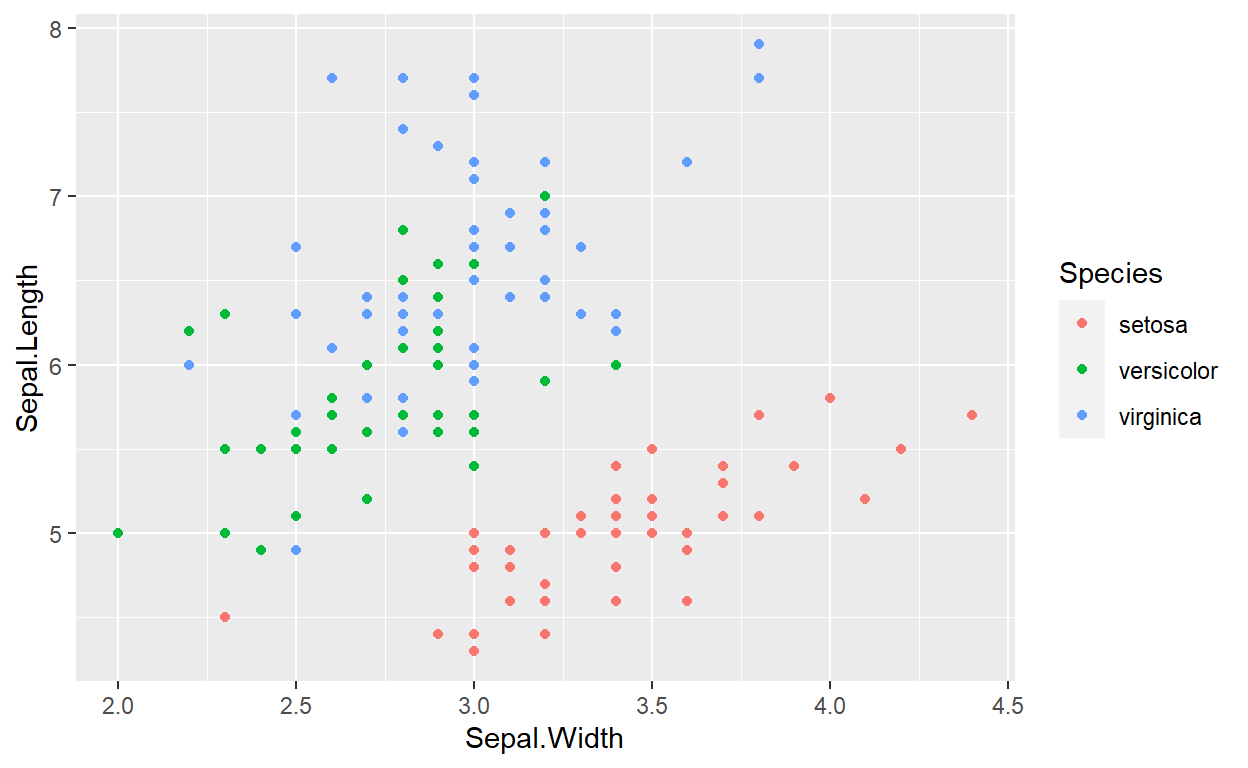
\includegraphics{figures/sepalwidthlength-1} 

}

\caption{Relation between sepal width and length in three species of Iris.}\label{fig:sepalwidthlength}
\end{figure}

When this file will be processed, it will create an image file (\texttt{figures/sepalwidthlength.png}) with the default dimension and the caption specified by the value of the \texttt{fig.cap} argument. You can use markdown formatting within the captions of your figures. This figure will have the label \texttt{fig:sepalwidthlength} that we will be able to use for cross referencing (see below).

If you wish to incorporate a figure that is not generated by code (a photo of your field site or study organism), using the function \texttt{\#knitr::include\_graphics()} takes care of many details for you, and generates labels and captions as if it was generated by code.

\begin{center}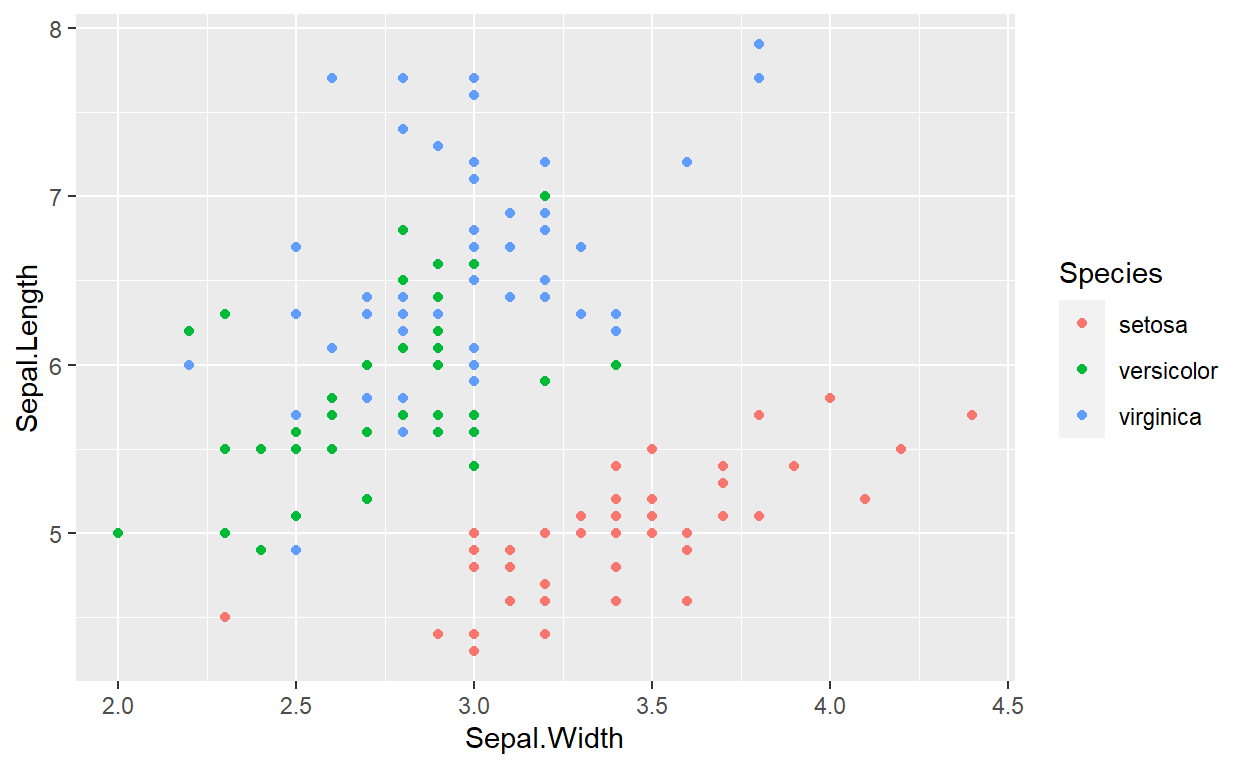
\includegraphics[width=17.33in]{figures/iris} \end{center}

\hypertarget{how-to-deal-with-tables}{%
\subsection{How to deal with tables?}\label{how-to-deal-with-tables}}

To generate tables, \texttt{knitr} comes with the function \texttt{kable} that might be sufficient to make simple tables to represent data frames within your report. However, there are many packages that provide more sophisticated approaches to display and format tabular data within your reports. This \href{https://hughjonesd.github.io/huxtable/design-principles.html}{page} provides an overview of the capabilities of the different packages.

\hypertarget{how-to-deal-with-citations}{%
\subsection{How to deal with citations?}\label{how-to-deal-with-citations}}

You need two things: a BibTeX file that contains all the citations you use in your manuscript and a CSL (Citation Style Language) file that specifies the format of your citation. Software citation managers such as Zotero or Mendeley provide options to generate BibTeX files for your citations. CSL files exist for most journals, and can be downloaded from: \url{https://www.zotero.org/styles}. This is a convenient search interface provided by Zotero but you do not need to use Zotero to download or use these files.

\hypertarget{where-can-i-find-more-information}{%
\section{Where can I find more information?}\label{where-can-i-find-more-information}}

\begin{itemize}
\tightlist
\item
  The RStudio Markdown website: \url{http://rmarkdown.rstudio.com/}
\item
  The bookdown website: \url{https://bookdown.org/yihui/bookdown/}
\end{itemize}

\hypertarget{documenting-and-managing-dependencies}{%
\chapter{Documenting and managing dependencies}\label{documenting-and-managing-dependencies}}

Reproducibility is also about making sure someone else can re-use your code to obtain the same results as yours. Understanding why your analysis may not lead to the same results on a different computer can be useful to determine how careful you need to be in documenting your setup.

For someone else to be able to reproduce the results included in your report, you need to provide more than the code and the data. You also need to document the exact versions of all the packages, libraries, and software you used, and potentially your operating system as well as your hardware.

R itself is very stable, and the core team of developer takes backward compatibility (that old code works with recent version of R) very seriously. However, default values in some functions have changed, and new functions get introduced regularly. If you wrote your code on a recent version of R and give it to someone who hasn't upgraded recently, they may not be able to run your code. If R itself is stable, the packages are generally much less stable. New functionalities get introduced with each versions, some functions get deprecated, and defaults options change. Code written for one version of a package may produce very different results with a more recent version.

Documenting and managing the dependencies of your project correctly can be a complicated. However, even simple documentation that helps others understand the setup you used can have a big impact. Here we present three levels of complexity to document the dependencies for your projects.

\hypertarget{show-the-packages-you-used}{%
\section{Show the packages you used}\label{show-the-packages-you-used}}

With R, the simplest (but useful and important) approach to document your dependencies is to report the output of \texttt{sessionInfo()} (or \texttt{devtools::session\_info()}). Among other information, this will show all the packages (and their versions) that are loaded in the session you used to run your analysis. If someone wants to recreate your analysis, they will know which packages they will need to install.

\hypertarget{use-packages-that-help-recreate-your-setup}{%
\section{Use packages that help recreate your setup}\label{use-packages-that-help-recreate-your-setup}}

The \texttt{checkpoint} package provides a way to download all the packages at a given date from CRAN. Thus, from the output provided by \texttt{sessionInfo()}, they could recreate your setup. It however makes two important assumptions: all your packages were up-to-date with CRAN at the time of your analysis; you were not using packages that are not available from CRAN (e.g.~the development version of a package directly from a git repository).

Another approach is to use the \texttt{packrat} package. This package creates a library (a collection of packages) directly within your analysis directory. It increases the size of your project as all the source code for the packages is included, but it ensures that someone can recreate more reliably the same environment as the one you used for your analysis. It also makes it easier because the installation of these packages is fully automated for the person wanting to have the same setup.

\hypertarget{use-containers-to-share-your-setup}{%
\section{Use containers to share your setup}\label{use-containers-to-share-your-setup}}

A step further in complexity is to use Docker. With Docker you recreate an entire operating system with all the software, data, and packages needed for your analysis. It is more technical to set up but it allows you to distribute the exact same environment as the one you used. If you want others to be able reproduce your results, and your analysis depends on software that can be difficult to install, it is an option that might be worth exploring.

  \bibliography{book.bib,packages.bib}

\end{document}
